\documentclass{ExcelAtFIT}
\usepackage[T1]{fontenc}
%\documentclass[czech]{ExcelAtFIT} % when writing in CZECH
%\documentclass[slovak]{ExcelAtFIT} % when writing in SLOVAK

%\todo{opravit citaci pro [3]}

%--------------------------------------------------------
%--------------------------------------------------------
%	REVIEW vs. FINAL VERSION
%--------------------------------------------------------

%   LEAVE this line commented out for the REVIEW VERSIONS
%   UNCOMMENT this line to get the FINAL VERSION
%\ExcelFinalCopy


%--------------------------------------------------------
%--------------------------------------------------------
%	PDF CUSTOMIZATION
%--------------------------------------------------------

\hypersetup{
	pdftitle={Evolution of programs controlling simple robot model},
	pdfauthor={Jakub Fajkus},
	pdfkeywords={Evolutionary computation, Linear Genetic Programming, Robotics}
}

%--------------------------------------------------------
%--------------------------------------------------------
%	ARTICLE INFORMATION
%--------------------------------------------------------

\ExcelYear{2018}

\PaperTitle{Evolution of programs controlling simple robot model}

\Authors{Jakub Fajkus*}
\affiliation{*%
  \href{mailto:xfajku06@stud.fit.vutbr.cz}{xfajku06@stud.fit.vutbr.cz},
  \textit{Faculty of Information Technology, Brno University of Technology}}

\Keywords{Evolutionary computation  --- Linear Genetic Programming --- Robotics}

\Supplementary{\href{http://youtu.be/S3msCdn3fNM}{Demonstration Video} --- \href{http://excel.fit.vutbr.cz/}{Downloadable Code}}


%--------------------------------------------------------
%--------------------------------------------------------
%	ABSTRACT and TEASER
%--------------------------------------------------------

\Abstract{
The aim of this work is to utilize Evolutionary Algorithms for finding a computer programs in order to control simple robot models.
A model is placed in the physical simulation where it is supposed to move along given specified reference points.
The program that controls the model consists of application specific instructions and its design is inspired by Linear Genetic Programming.
The program has an information about a direction to the next reference point.
}

\Teaser{
	\TeaserImage{placeholder.pdf}
	\TeaserImage{placeholder.pdf}
	\TeaserImage{placeholder.pdf}
}



%--------------------------------------------------------
%--------------------------------------------------------
%--------------------------------------------------------
%--------------------------------------------------------
\begin{document}

\startdocument


%--------------------------------------------------------
%--------------------------------------------------------
%	ARTICLE CONTENTS
%--------------------------------------------------------

%--------------------------------------------------------
%--------------------------------------------------------
%--------------------------------------------------------
%--------------------------------------------------------
\section{Introduction}
In the area of robotics it is very important to be able to create prototypes quickly and cheaply.
For this purpose it is beneficial to use computer models and simulation when designing the \todo{structure?} of the robot.
There are many ways to control the robot depending on the given requirements.
It can be, for example, controlled by instructions of an imperative language~\cite{Wolff2007}, finite state machines~\cite{Hodgins1996}, classical control theory~\cite{Mita1984} or artificial neural networks~\cite{Reil2002}~\cite{Lewis1996}.
For a fast prototyping we can use Evolutionary Algorithms to evolve the robot control.

The problem to solve in this work is defined as follows.
We have a model of a simple robot and we want to evolve a program that is based on instructions of an imperative language.
The robot is supposed to move in a simulated environment and visit the predefined reference points.
The reference points, specified by the designer, define a trajectory the robot should follow.
The program that controls the model is being evolved using Evolutionary Algorithms and then evaluated in the Mujoco simulator~\cite{Todorov2012}.

There is a number of works using Evolutionary Algorithms to evolve controllers based on artificial neural networks~\cite{Randall1992}~\cite{Farooq2013}.
There are also works that are using Genetic Programming~\cite{Macedo2017}.
The most similar work to to this one is the work of Wolff and Wahde~\cite{Wolff2007}.
They are using Linear Genetic Programming to evolve a bipedal locomotion of a humanoid model.

The research conducted in this paper is primarily motivated by~\cite{Wolff2007} where a successful evolution of
control algorithms was proposed for a specific humanoid model. In this paper we present an extended concept which allows evolutionary
design of controllers for various creatures with different number of legs. The goal is to evolve a program using a very reduced intruction
set in which several sub-programs can be evolved automatically and simultaneously in order to perform specific motions of the model.
Our approach will be evaluated using several trajectories the model should follow in a simulated environment. The detail of the proposed
system will be described in Section \todo{ref na vysvetleni v sekci}

%--------------------------------------------------------
%--------------------------------------------------------
%--------------------------------------------------------
%--------------------------------------------------------
\section{Linear Genetic Programming}
\label{sec:theory}
Here we will discuss a brief introduction to Linear Genetic Programming (LGP), based on~\cite{Brameier2010}.
LGP is a special variant of the Genetic Programming\todo{Jon Koza}.

Genetic Programming (GP) solves a modelling problem.
That means we know a set of inputs to a system and the outputs it should produce.
But we do not have the system that will compute the inputs and tell us the output.
When solving a control problem, we are looking for such a function, that will lead to the desired behavior.

In GP we are evolving computer program $P$ that represents a function: $f : I^n \to O^m$, where $I^n$ denotes the n-dimensional input data and $O^m$ denotes the m-dimensional output data.

The genotype space $G$ in GP includes all programs that can be composed of elements of a given programming language $L$.
The programming language $L$ is defined by an instruction set and a terminal set.
An interpreter translates the genotype representation into the phenotype, i.e.\ the behavior of the robot.
The phenotype is then executed and it's fitness is evaluated using a software physical simulator.
\todo{fitness se meri metodou nejmensich ctvercu! - nekam s tim :D}

The original GP uses trees that correspond to expressions from a functional programming language.
The nodes of the tree represent functions, while leaves represent input values or constants.

The Linear Genetic Programming is a variant where the programs are composed of a sequence of instructions from an imperative language or a machine code.
Each program has available a predefined set of registers that can hold constants as well as results of instructions.
Those registers are often divided into groups: input registers, output registers and calculation registers.
The instructions are composed of an operation and one or more operands.
The operands may be registers or constants.
As the program is being executed it modifies the values of the registers, reads the inputs and writes the outputs.

%--------------------------------------------------------
%--------------------------------------------------------
%--------------------------------------------------------
%--------------------------------------------------------

\section{Evolution of Robot Controller using LGP}
\label{sec:ExperimentsSetup}
In order to evolve a robot controller, the LGP concept was combined with an evolutionary algorithm and the Mujoco simulator\cite{Todorov2012} was used to evaluate the candidate programs using a built-in interpreter.
There is a prepared scene in the simulator containing a set of reference points defining a spiral (Figure~\ref{fig:SpiralTop}).
The robot model is given a task (using the evolved LGP programs) to move from point to point at given order and to get as close as possible to each of them.
This way the robot moves on a predefined trajectory.

%todo: image placement
%todo: change the image to containt he 3 leg thingy and where the reference points are not all over the place
\begin{figure}[t]
\centering
{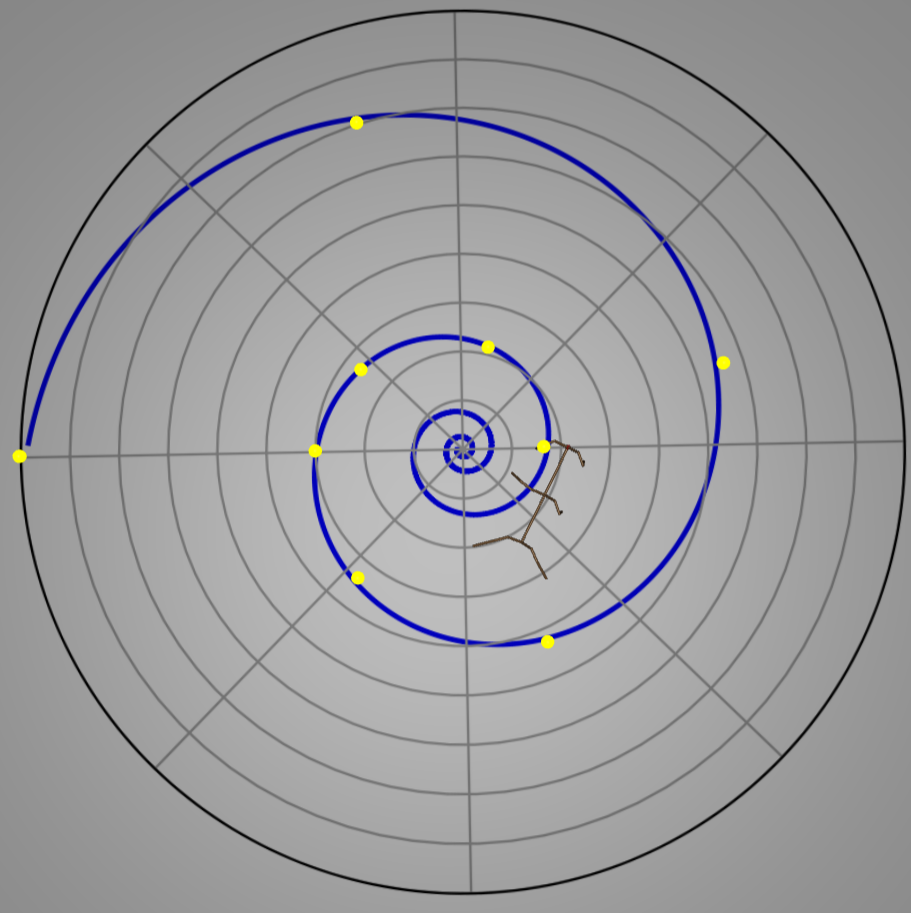
\includegraphics[height=19em]{spiral_top_v2.png}}
\caption{Top view at the scene in the simulator.
We can see a spiral on which are placed the reference points (yellow spheres).
The robot's model is brown.
}
\label{fig:SpiralTop}
\end{figure}

\todo{vlozit obrazek detailu robota a popsat jej}

\subsection{LGP-Based Robot Controller}
\label{subsec:lgp-basedRobotController}
The programs (which are the subject of evolution using LGP) are composed of application-specific instruction of the form \texttt{COPY ARG1 ARG2}, where \texttt{COPY} is the instruction name, \texttt{ARG1} is source register and \texttt{ARG2} is the destination register.
Each register has it's unique identification called \textit{index} which is used in a instruction's argument.
As the program is being executed, it copies values from input or constant registers into the output registers.

The interpreter has 11 constant registers (indices 0–10) holding integer values from -5 to 5, 2 input registers (indices 11–12) and 3 output registers (indices 13–15).
The values of the input registers depend on the direction to the next reference point.
Each output register is connected with exactly one robot's joint and it's value is converted into a force that is applied in the joint.

For the purposes of this work a concept of subprograms has been introduced which works as follows.

The individual's genotype (representing the whole program) is split into 3 smaller subprograms - \textit{init}, \textit{event} and \textit{main}.

The \textit{main} subprogram is being run in an endless loop during the simulation.
Only one instruction is executed at a time.
Period of 0.3 seconds between instructions is used.

The \textit{init} subprogram is executed at the start of the simulation and its purpose is to set the initial rotation of all robot's joints.
All instructions of the init program are executed in a single time.
After that, the main subprogram is paused for one second to give the robot's joints time to finish the rotation.

The \textit{event} subprogram is run each time the robot gets close enough to some of the reference points (but only once for each point).
It's purpose is to change the robot's joints rotation as a preparation to move to the next reference point.
The event subprogram is executed in a single time and the main subprogram is paused as well as in the \textit{init} subprogram.

A schema of the interpreter is at Figure~\ref{fig:Interpret}.
Each 0.3 seconds a instruction from the \textit{main} subprogram is executed.
The first argument is an input or constant register index, the other one is the output register index.
A value from constant or input register is then copied into the output register.

Each of the interpret's output registers is mapped to exactly one robot's joint.
Each time an instruction is executed, the values from the output registers are read.
The values are then used as a control signal to the simulator for each joint in the model.
A value (control signal) holds two pieces of information.
The sign of the value is used to determine the direction of the force applied (clockwise, counterclockwise).
The absolute value of the number is used to determine the \todo{magnitude} of the force.
Based on those signals and the model parameters the simulator calculates a force that will be applied in the joint.


%todo: image placement
\begin{figure}[t]
	\centering
	{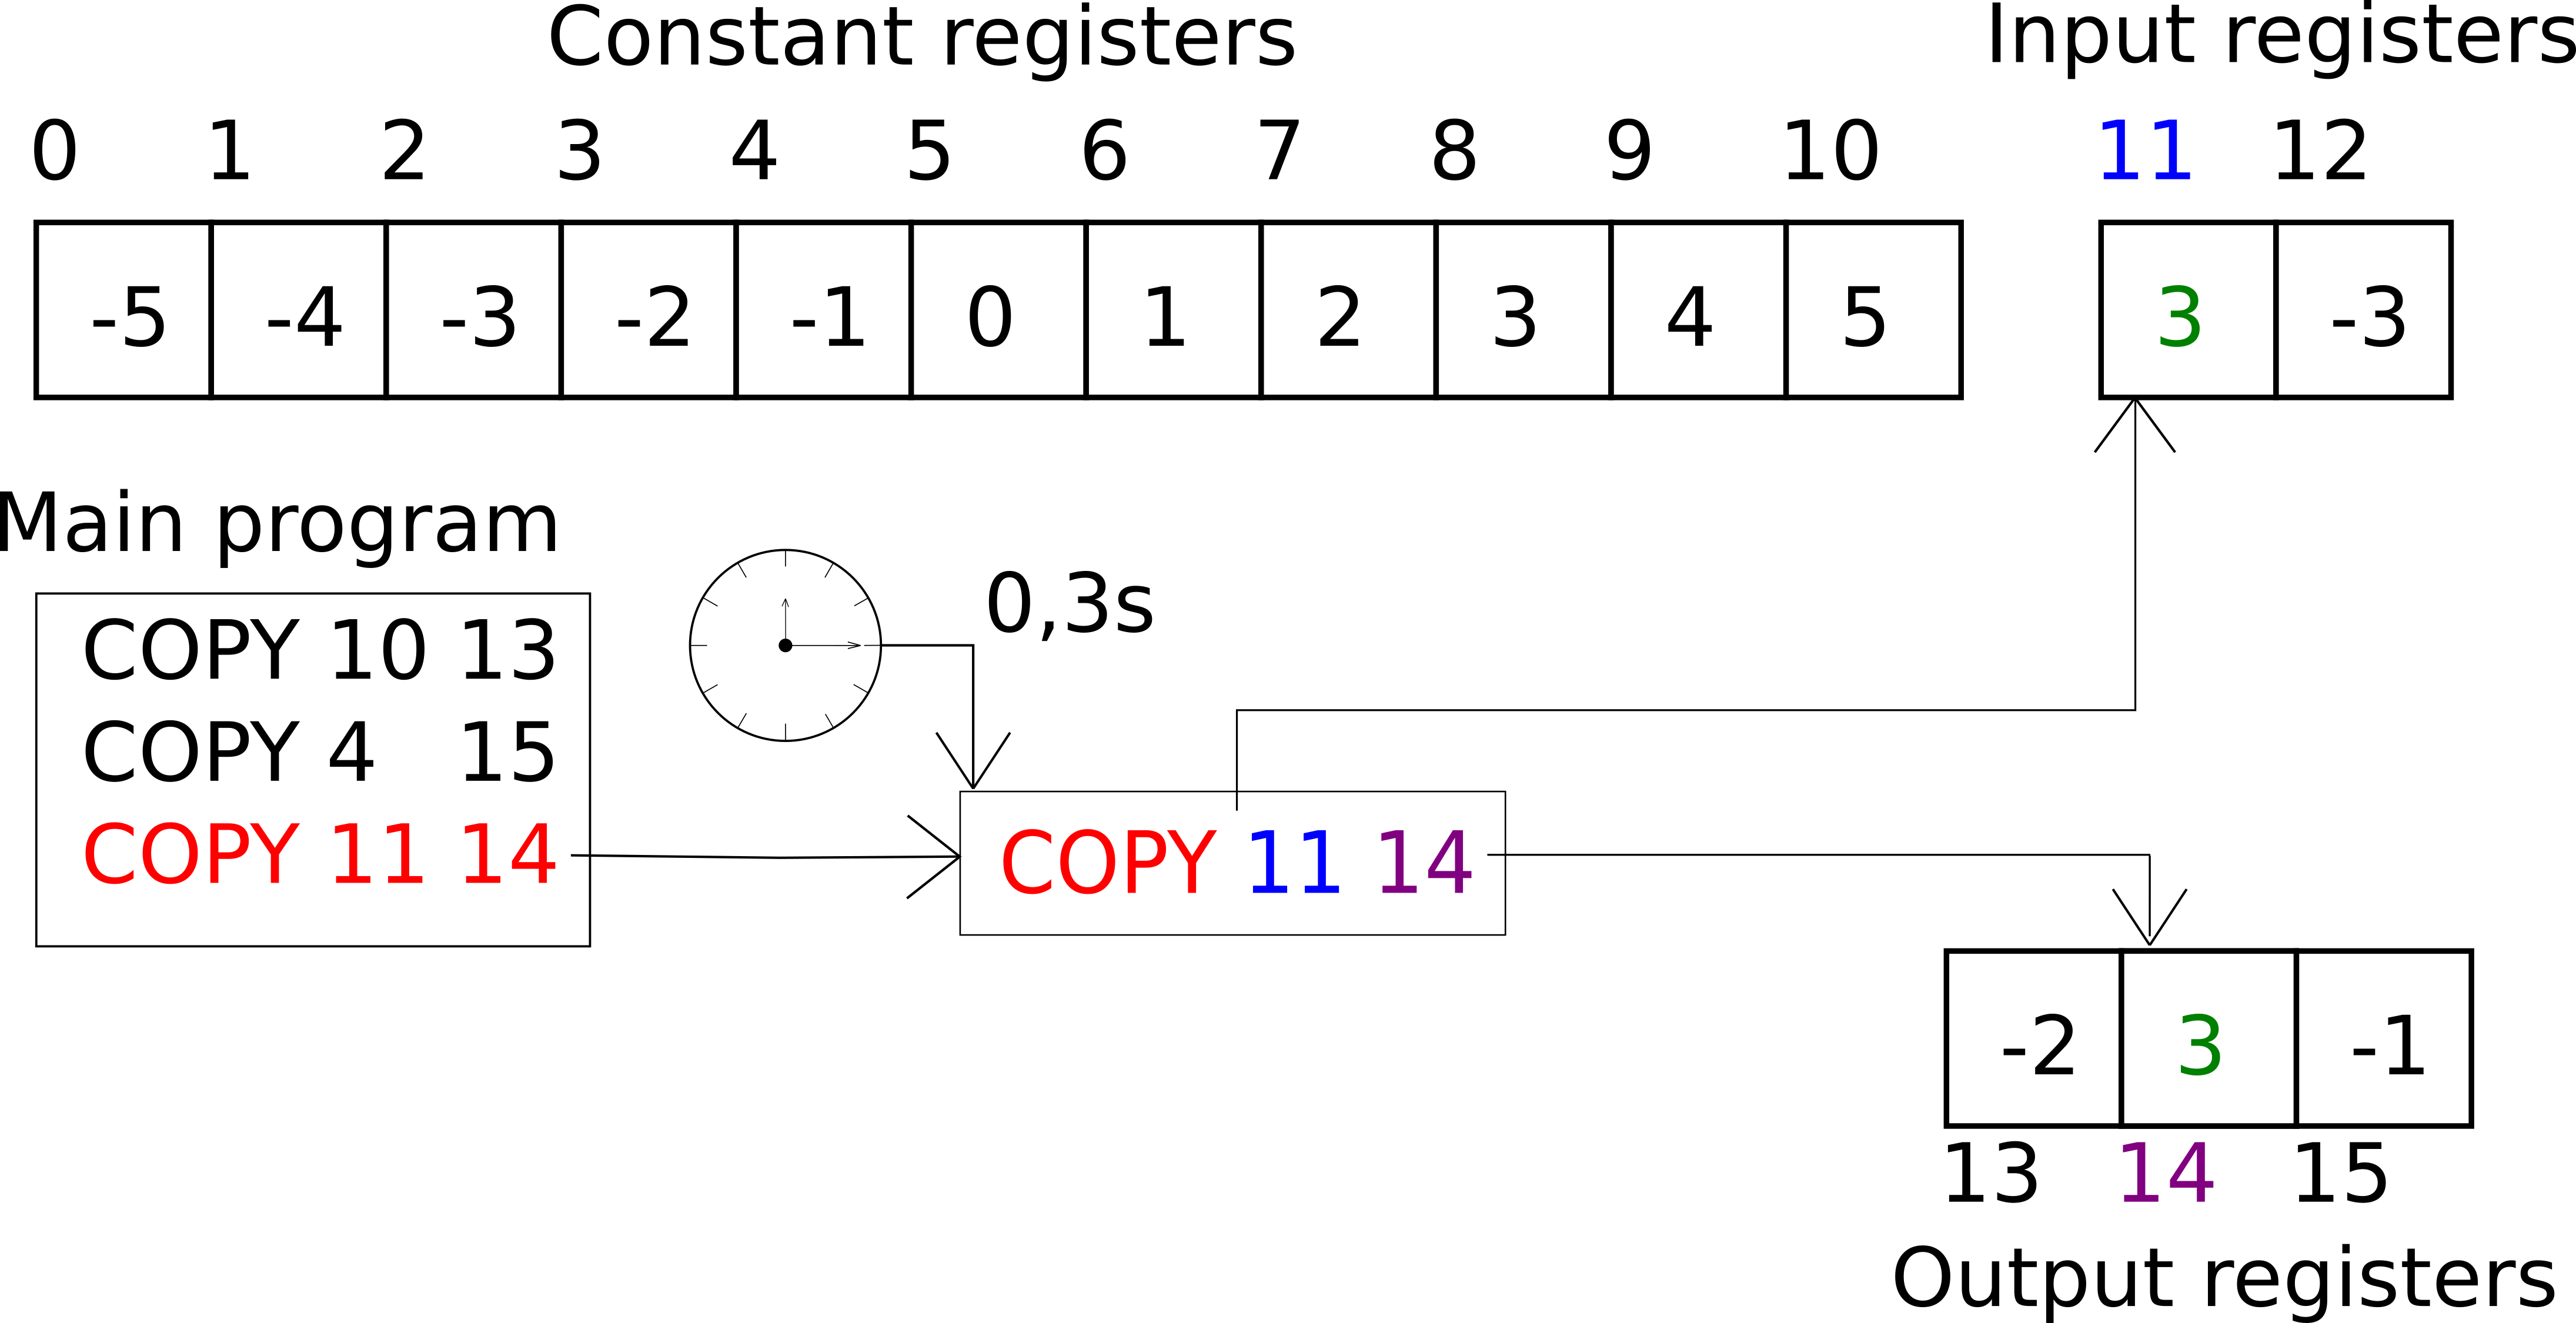
\includegraphics[width=20em]{interpret.png}}
	\caption{
	Schematic view of the interpreter.
	The situation depicted there is as follows.
	The instruction to be executed has arguments with values of 11 and 14.
	A value from input register with index 11 is copied into the output register with index 14.
	}
	\label{fig:Interpret}
\end{figure}



%--------------------------------------------------------
%--------------------------------------------------------
%--------------------------------------------------------
%--------------------------------------------------------
\subsection{Evolution of robot controllers}
\label{sec:EvolutionOfRobotControllers}
In order to design the LGP-based programs to control the robot, a simple steady-state Genetic Algorithm (GA) was applied -- see Figure XXX
\todo{(pseudokod jednoducheho steady-state GA - viz moje DP)}.

The parameters of the GA are as follows.
\begin{itemize}
	\item Population size is set to 1000
	\item Steady-state population model is used (the better half of the population is kept, the other one replaced).
	\item The genotype length is fixed to 36 instructions.
	\item A custom genetic crossover based on uniform crossover is used (Figure~\ref{fig:Crossover}).
	\item The probability of crossover is 80\%.
	\item The mutation is set with 100\% probability and changes only one gene.
	\item Parent selection is implemented by tournament of size 2.
\end{itemize}


Each chromosome in the GA represents a single program (a candidate controller for the robot).
The structure of the chromosome is illustrated in Figure XXX
The chromosome has fixed length (36 genes).
It is split into three smaller subprograms(init, event, main) that have fixed lengths, too.
Each gene represents a single instruction.
The instruction is a triplet and consists of the instruction name and two numbers.

The GA applies both the crossover and mutation operators which work as follows.
The crossover operates on the level of subprograms.
It is based on the uniform crossover with $p = 0.5$ but instead of swapping the genes, it swaps the whole subprograms (Figure~\ref{fig:Crossover}).

The mutation operates on the level of genes~(instructions).
There is a 80\% chance of mutating the instruction values.
There is a 20\% chance of replacing the instruction with a new, randomly generated one.
When mutating the instruction values, there is en equal chance to mutate the first or the second argument.
The mutation of the values is implemented as a generating a random value from the specified range of values.

The fitness evaluation of the candidate programs is performed as follows.
For each program a new simulation is run.
During the simulation, the program is being executed and it controls the robot's model (as explained in the previous section).
Every second of the simulation, the distance between the robot and each of the reference points is recorded.
The program fitness is then calculated as the \todo{nejmensi ctverce}.
This way, the evolution minimizes the minimal distance between the robot and each of the reference points.
\todo{napr. zkusit naimplementovat metodu nejmensich ctvercu, at jsme presni a nevymyslime si vysledky}


%todo: image placement
\begin{figure}[t]
	\centering
	{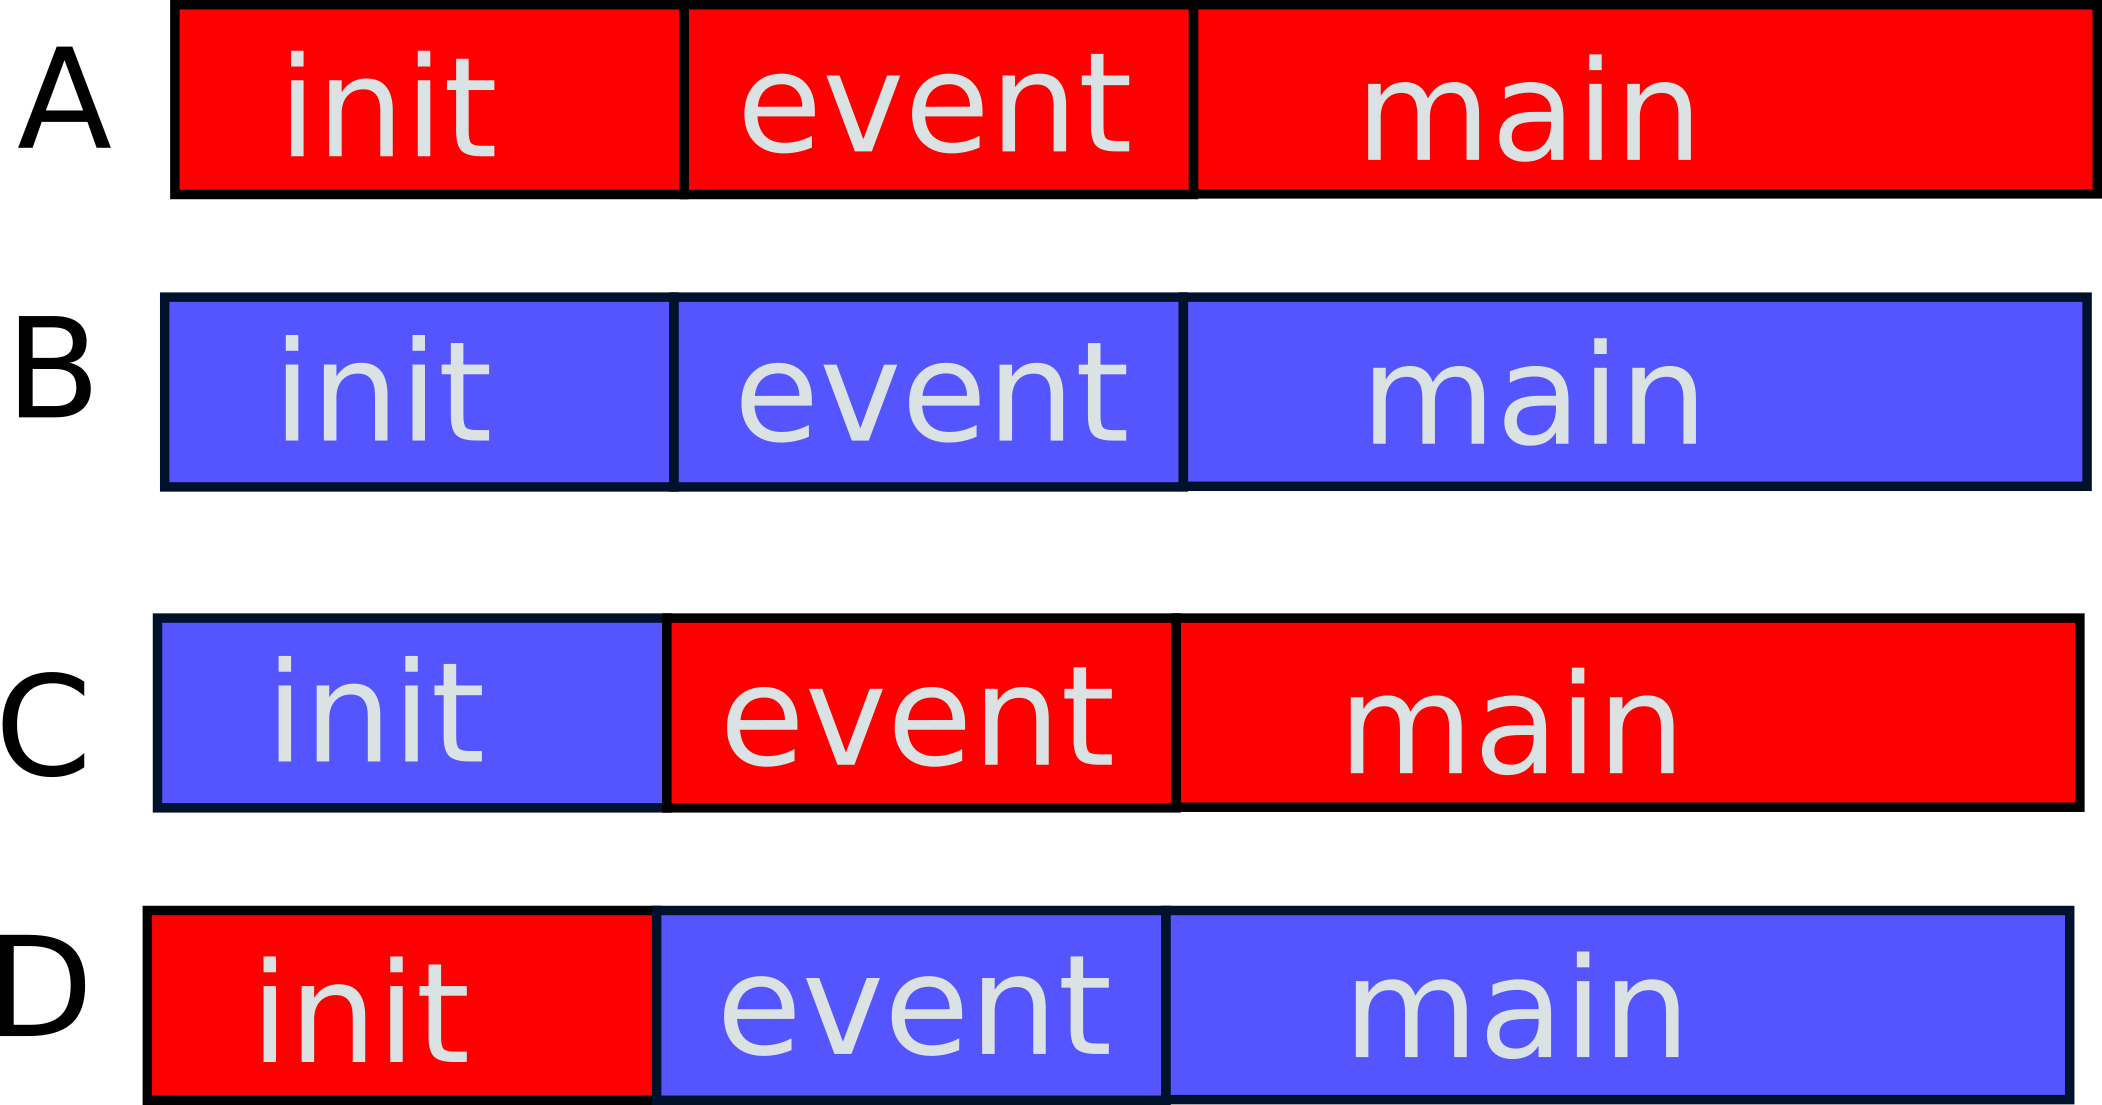
\includegraphics[width=18em]{crossover.png}}
	\caption{
	A custom genetic crossover is used.
	It is based on uniform crossover, but it operates on the subprograms level.
	The genome of parents is divided into the subprograms and then there is a 1:1 chance to to inherit the subprogram from parent A or B.
	Here, the crossover of parents A and B resulted into offsprings C and D.
	In this case, only the init subprograms were swapped.
	}
	\label{fig:Crossover}
\end{figure}



%--------------------------------------------------------
%--------------------------------------------------------
%--------------------------------------------------------
%--------------------------------------------------------

\section{Results}
The evolution was run 20 times.
The typical progress of fitness values can be seen in Figure~\ref{fig:FitnessGraph}.
The maximum fitness possible in the given amount of time is around 280 and the best solution found had 255.9.

Some of the best results were evaluated for a different trajectories (Figure~\ref{fig:PostExperimentTests}), however the behaviour was not satisfying.
They definitely exhibited some degree of movement towards the reference points, but the locomotion pattern encoded in the program was not flexible enough to cope with different environment.
This is mainly because the locomotion pattern is expressed as a list of hardcoded instructions with constant values.
So, if the training environment had the reference points placed on a spiral, the program itself is evolved to move generally in a spiral.

If a different approach was used, for example using more input values coming either from oscillators with different frequencies or some sensory information (rotation of joints), the programs could then evolve a universal locomotion pattern that would be only adjusted with the information about direction to the next reference point.

%todo: image placement
\begin{figure}[t]
	\centering
	{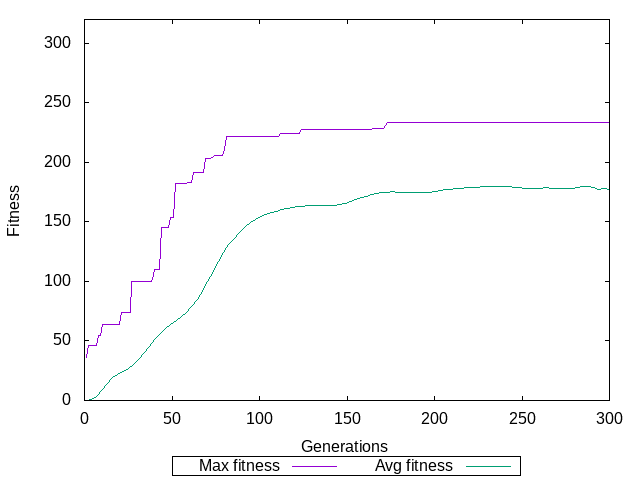
\includegraphics[height=17em]{runFitnessGraph.png}}
	\caption{
	A typical progress of fitness values in a evolutionary run.
	}
	\label{fig:FitnessGraph}
\end{figure}

%todo: image placement
\begin{figure}[t]
	\centering
	{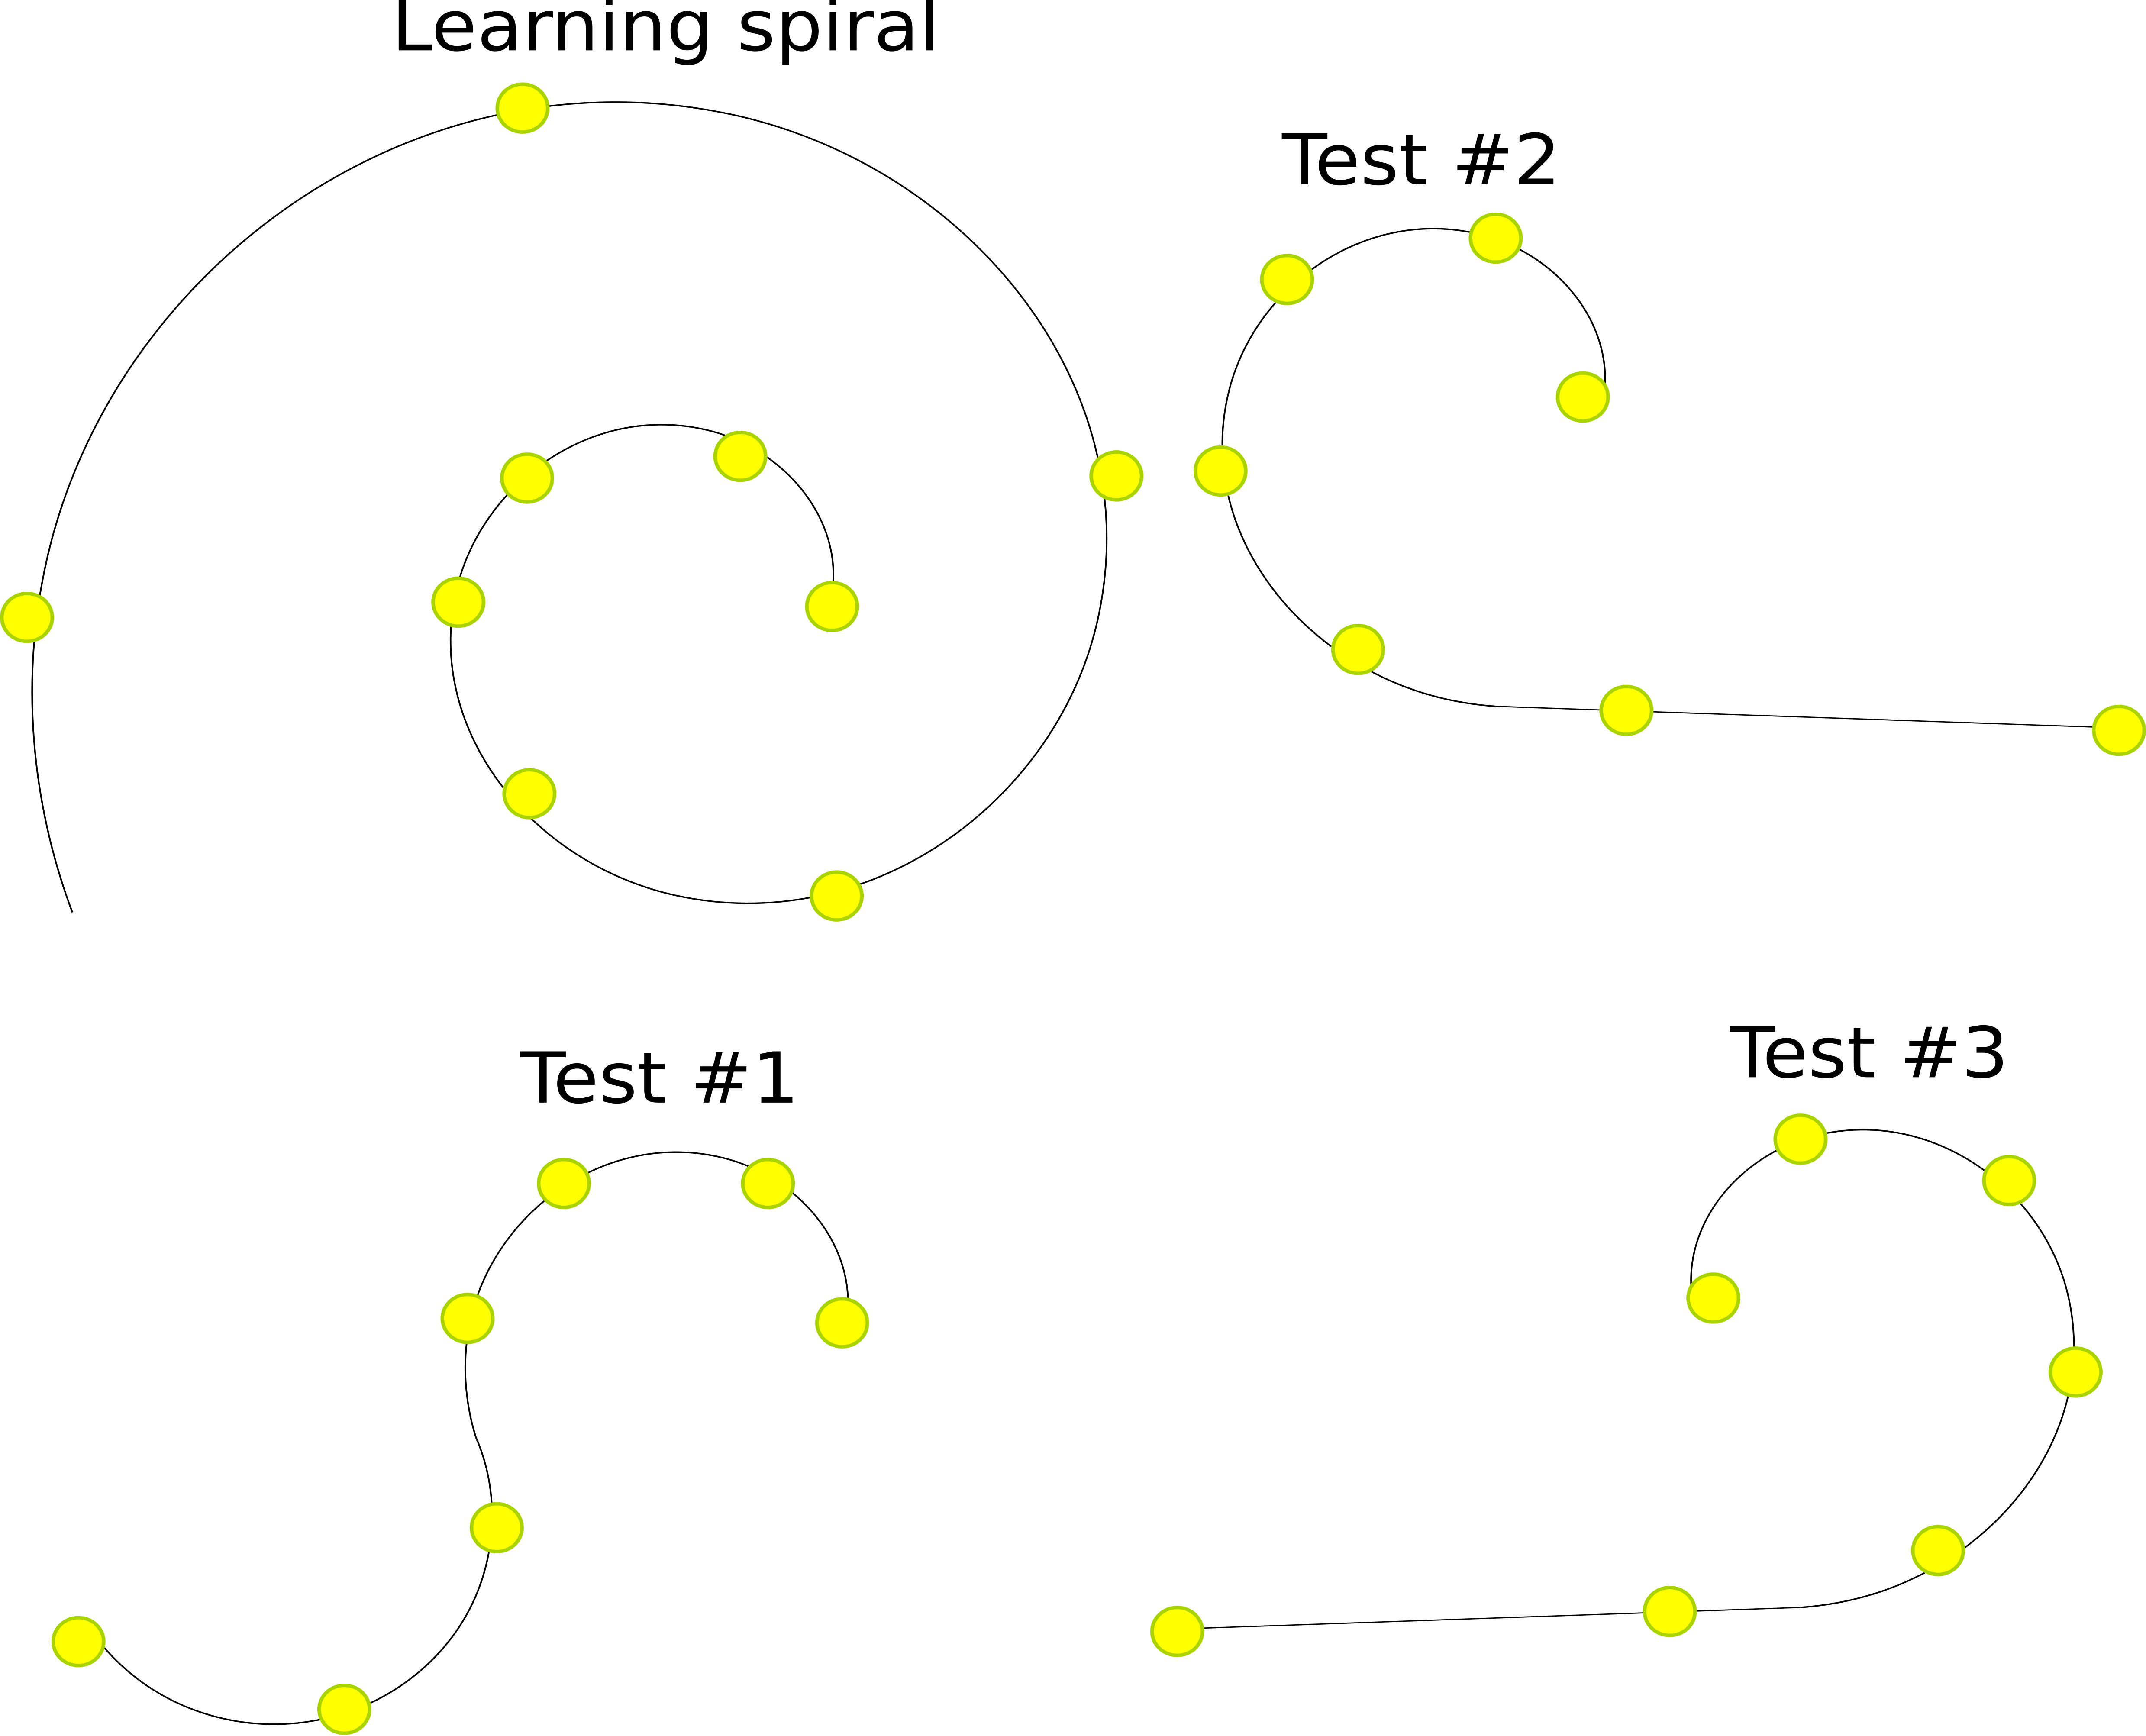
\includegraphics[height=16em]{postExperimentTests.png}}
	\caption{
	Trajectories used to evaluate the ability of the found solutions to navigate in unknown conditions.
	}
	\label{fig:PostExperimentTests}
\end{figure}

%--------------------------------------------------------
%--------------------------------------------------------
%--------------------------------------------------------
%--------------------------------------------------------

\section{Conclusions}
\label{sec:Conclusions}

%\textbf{[Paper Summary]} What was the paper about, then? What the reader needs to remember about it?
This work showed an usage of Evolutionary Algorithms for finding a program for a robot control.
The results show that the programs evolved successfully to meet the given criteria, although failed to adapt to a new behaviour.
However, the original question behind this work was that whether a very simple program could control the robot in a way that it will move on a non trivial trajectory.

Providing the program with more sensory information as well as some oscillators could lead to better universality.
This thought will be put under test in the future experiments.

%\textbf{[Highlights of Results]} Exact numbers. Remind the reader that the paper matters.
%\phony{Lorem ipsum dolor sit amet, consectetur adipiscing elit. Sed tempus fermentum ipsum at venenatis. Curabitur ultricies, mauris eu ullamcorper mattis, ligula purus dapibus mi, vel dapibus odio nulla et ex. Sed viverra cursus mattis. Suspendisse ornare semper condimentum. Interdum et malesuada fames ac ante ipsum.}
%
%\textbf{[Paper Contributions]} What is the original contribution of this work? Two or three thoughts that one should definitely take home.
%\phony{Lorem ipsum dolor sit amet, consectetur adipiscing elit. Praesent posuere mattis ante at imperdiet. Cras id tincidunt purus. Aliquam erat volutpat. Morbi non gravida nisi, non iaculis tortor. Quisque at fringilla neque.}
%
%\textbf{[Future Work]} How can other researchers / developers make use of the results of this work?  Do you have further plans with this work? Or anybody else?
%\phony{Lorem ipsum dolor sit amet, consectetur adipiscing elit. Suspendisse sollicitudin posuere massa, non convallis purus ultricies sit amet. Duis at nisl tincidunt, maximus risus a, aliquet massa. Vestibulum libero odio, condimentum ut ex non, eleifend.}

%todo: podekovani!
%\section*{Acknowledgements}
%I would like to thank my supervisor X. Y. for his help.

%--------------------------------------------------------
%--------------------------------------------------------
%--------------------------------------------------------
%	REFERENCE LIST
%--------------------------------------------------------
%--------------------------------------------------------
\phantomsection
\bibliographystyle{unsrt}
\bibliography{2018-ExcelFIT-ShortName-bib}

%--------------------------------------------------------
%--------------------------------------------------------
%--------------------------------------------------------
\end{document}
